\documentclass[10pt,a4paper]{article}

\usepackage[utf8]{inputenc}
\usepackage[T1]{fontenc}
\usepackage{lmodern}
\usepackage[margin=0.65in,top=0.60in,bottom=0.60in]{geometry}
\usepackage{amsmath,amssymb,amsfonts}
\usepackage{booktabs}
\usepackage{array}
\usepackage{multirow}
\usepackage{tabularx}
\usepackage{xcolor}
\usepackage{graphicx}
\usepackage{pgfplots}
\pgfplotsset{compat=1.18}
\usepackage{enumitem}
\usepackage{titlesec}
\usepackage{hyperref}
\usepackage{fancyhdr}
\usepackage{caption}

\definecolor{navy}{RGB}{18,53,105}
\definecolor{crimson}{RGB}{175,28,45}
\definecolor{forest}{RGB}{27,120,55}
\definecolor{slate}{RGB}{85,95,110}
\definecolor{purpleaccent}{RGB}{118,68,138}
\definecolor{boxbg}{RGB}{246,248,252}

\hypersetup{
    colorlinks=true,
    linkcolor=navy,
    citecolor=navy,
    urlcolor=navy
}

\titlespacing*{\section}{0pt}{6pt plus 2pt minus 1pt}{3pt plus 1pt minus 1pt}
\titlespacing*{\subsection}{0pt}{5pt plus 1pt minus 1pt}{2pt plus 1pt minus 1pt}
\titlespacing*{\subsubsection}{0pt}{3.5pt plus 1pt minus 1pt}{1.5pt plus 1pt minus 1pt}
\setlength{\parindent}{0pt}
\setlength{\parskip}{2.8pt}
\setlist[itemize]{leftmargin=1.4em,itemsep=1pt,topsep=1.5pt}
\setlist[enumerate]{leftmargin=1.5em,itemsep=1pt,topsep=1.5pt}
\captionsetup{font=small,labelfont=bf,skip=3pt}

\pagestyle{fancy}
\fancyhf{}
\lhead{\footnotesize CS 5326: Advanced Generative AI and Agents}
\rhead{\footnotesize PA 3: Search over Reasoning \& Step-Level PRMs}
\cfoot{\footnotesize\thepage}
\renewcommand{\headrulewidth}{0.4pt}

\begin{document}

\begin{center}
    {\Large\bfseries CS 5326: Advanced Generative AI and Agents}\\[3pt]
    {\large\bfseries Programming Assignment 3: Search over Reasoning and Step-Level Process Reward Models}\\[5pt]
    {\small \textbf{Name:} Muhammad Ammar \quad|\quad \textbf{Roll Number:} 25280019 \quad|\quad \textbf{GitHub:} \url{https://github.com/Ammar946/cs5326-pa3}}
\end{center}
\vspace{-4pt}
\noindent\rule{\textwidth}{0.6pt}
\vspace{-6pt}

\section{Benchmark Results and Scaling Curves}

\subsection{Comparative Evaluation Across Decoding and Search Strategies}
\sloppy
We evaluate six mandatory inference-time configurations plus the optional continuous-logit bonus (\texttt{product\_logprob}) over the fixed 50-problem GSM8K benchmark (\texttt{data/gsm8k\_test\_50.jsonl}) using an asymmetric policy-verifier architecture on Kaggle dual T4 GPUs: \texttt{Qwen/Qwen2.5-1.5B-Instruct} in \texttt{float16} (\texttt{cuda:0}) as the generator policy $\pi_\theta$ and \texttt{Qwen/Qwen2.5-7B-Instruct} in 4-bit NormalFloat (\texttt{NF4}, \texttt{cuda:1}) as the step-level Process Reward Model (PRM) verifier $f_\phi$. To ensure a controlled evaluation, Self-Consistency at $N=5$ (\textbf{SC@5}) and all PRM Best-of-5 variants share the exact same pool of 5 temperature-sampled trajectories per problem ($T=0.7, p=1.0, k=0$), while Compute-Matched Self-Consistency (\textbf{SC@15}) retains those 5 trajectories (indices $0\dots 4$) and draws 10 additional samples (indices $5\dots 14$). Table~\ref{tab:summary} presents the complete empirical summary alongside 95\% bootstrap confidence intervals ($1{,}000$ resamples over the 50 problems with seed $5326$).

\begin{table}[h!]
\centering
\caption{Empirical benchmark results across all 50 GSM8K test problems (\texttt{outputs/results\_summary.json} and \texttt{outputs/bonus\_product\_logprob.json}). Across 250 shared candidate paths, the 7B judge evaluated $1{,}042$ parsed reasoning steps ($\bar{K} = 4.168$ steps/candidate). 95\% Confidence Intervals (CI) are computed via 1,000 bootstrap resamples (seed 5326).}
\label{tab:summary}
\resizebox{\textwidth}{!}{%
\begin{tabular}{lccccccc}
\toprule
\textbf{Method} & \textbf{Acc. (\%)} & \textbf{95\% Boot. CI} & \textbf{Gen Calls} & \textbf{Judge Calls} & \textbf{Total Calls} & \textbf{Avg Gen / Judge Tok} & \textbf{Time (s)} \\
\midrule
Greedy ($N=1$) & 66.00 & $[52.0, 78.0]$ & 50 & 0 & 50 & $218.80 \;/\; 0.00$ & 477.08 \\
Self-Consistency ($N=5$) & 72.00 & $[60.0, 84.0]$ & 250 & 0 & 250 & $922.32 \;/\; 0.00$ & 556.61 \\
Compute-Matched SC ($N=15$) & 76.00 & $[62.0, 86.0]$ & 750 & 0 & 750 & $2828.26 \;/\; 0.00$ & 1250.33 \\
\midrule
\textbf{PRM Best-of-5 (\texttt{min})} & \textbf{80.00} & $[68.0, 90.0]$ & 250 & 1042 & 1292 & $922.32 \;/\; 620.06$ & 3037.35 \\
PRM Best-of-5 (\texttt{product}) & 72.00 & $[58.0, 84.0]$ & 250 & 1042 & 1292 & $922.32 \;/\; 620.06$ & 3037.35 \\
\textbf{PRM Best-of-5 (\texttt{step\_penalty}, $\lambda=2.0$)} & \textbf{80.00} & $[68.0, 90.0]$ & 250 & 1042 & 1292 & $922.32 \;/\; 620.06$ & 3037.35 \\
PRM Best-of-5 (\texttt{product\_logprob}) \textit{[Bonus]} & 78.00 & $[66.0, 88.0]$ & 250 & 1042 & 1292 & $922.32 \;/\; 620.06$ & 3037.35 \\
\bottomrule
\end{tabular}%
}
\end{table}

\subsection{Test-Time Scaling Curves: LLM Calls vs. Output Token Expenditure}
Figure~\ref{fig:scaling} plots exact-match accuracy across two complementary test-time compute axes: \textbf{(a) Total LLM Calls} (generation calls + step-level judge calls across all 50 problems) and \textbf{(b) Average Output Tokens per Problem} ($\text{generated\_tokens} + \text{judge\_tokens}$). Under pure majority-voting Self-Consistency (\texttt{outputs/sc\_scaling\_curve.json}), accuracy rises monotonically from $68.0\%$ at $N=1$ ($174.48$ tok/prob) to $74.0\%$ at $N=4$, dips slightly to $72.0\%$ at $N=5$ due to tie-breaking on a 5-sample pool, reaches a plateau of $80.0\%$ at $N \in \{9, 10, 11\}$ ($1{,}682.54$--$2{,}059.08$ tok/prob), and subsequently regresses to $76.0\%$ at $N \in \{14, 15\}$ ($2{,}828.26$ tok/prob) as repeated sampling reinforces high-frequency systematic misconceptions of the 1.5B generator.

\begin{figure}[h!]
\centering
\begin{minipage}{0.485\textwidth}
\centering
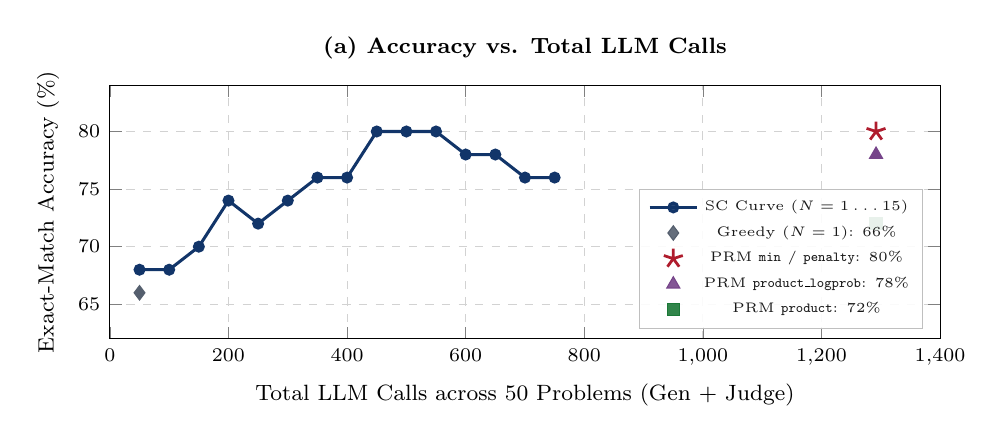
\begin{tikzpicture}
\begin{axis}[
    width=\textwidth,
    height=4.8cm,
    xlabel={\footnotesize Total LLM Calls across 50 Problems (Gen + Judge)},
    ylabel={\footnotesize Exact-Match Accuracy (\%)},
    title={\footnotesize\bfseries (a) Accuracy vs. Total LLM Calls},
    xmin=0, xmax=1400,
    ymin=62, ymax=84,
    grid=major,
    grid style={dashed,gray!35},
    tick label style={font=\scriptsize},
    legend style={font=\tiny, at={(0.98,0.04)}, anchor=south east, fill=white, fill opacity=0.9, draw=gray!50},
]
\addplot[color=navy, mark=*, mark size=1.6pt, line width=1.1pt] coordinates {
    (50,68.0) (100,68.0) (150,70.0) (200,74.0) (250,72.0)
    (300,74.0) (350,76.0) (400,76.0) (450,80.0) (500,80.0)
    (550,80.0) (600,78.0) (650,78.0) (700,76.0) (750,76.0)
};
\addlegendentry{SC Curve ($N=1\dots 15$)}

\addplot[only marks, color=slate, mark=diamond*, mark size=2.6pt] coordinates {(50,66.0)};
\addlegendentry{Greedy ($N=1$): 66\%}

\addplot[only marks, color=crimson, mark=star, mark size=3.6pt, line width=1pt] coordinates {(1292,80.0)};
\addlegendentry{PRM \texttt{min} / \texttt{penalty}: 80\%}

\addplot[only marks, color=purpleaccent, mark=triangle*, mark size=2.7pt] coordinates {(1292,78.0)};
\addlegendentry{PRM \texttt{product\_logprob}: 78\%}

\addplot[only marks, color=forest, mark=square*, mark size=2.2pt] coordinates {(1292,72.0)};
\addlegendentry{PRM \texttt{product}: 72\%}
\end{axis}
\end{tikzpicture}
\end{minipage}
\hfill
\begin{minipage}{0.485\textwidth}
\centering
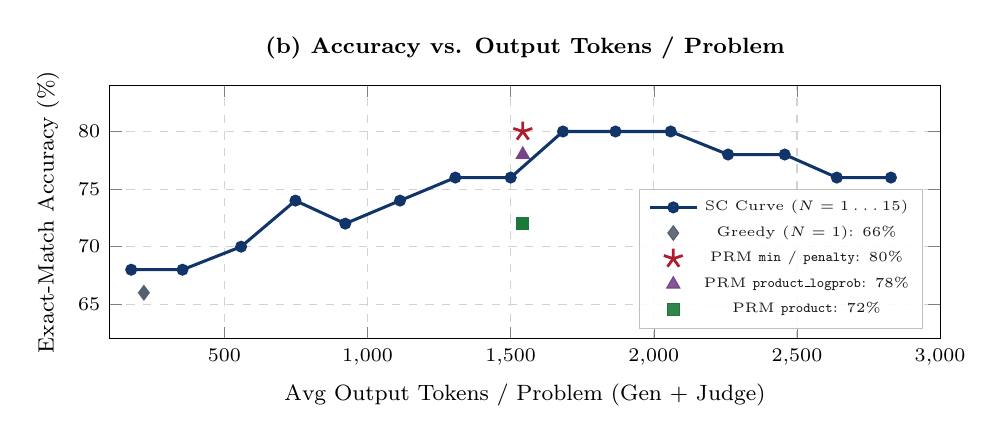
\begin{tikzpicture}
\begin{axis}[
    width=\textwidth,
    height=4.8cm,
    xlabel={\footnotesize Avg Output Tokens / Problem (Gen + Judge)},
    ylabel={\footnotesize Exact-Match Accuracy (\%)},
    title={\footnotesize\bfseries (b) Accuracy vs. Output Tokens / Problem},
    xmin=100, xmax=3000,
    ymin=62, ymax=84,
    grid=major,
    grid style={dashed,gray!35},
    tick label style={font=\scriptsize},
    legend style={font=\tiny, at={(0.98,0.04)}, anchor=south east, fill=white, fill opacity=0.9, draw=gray!50},
]
\addplot[color=navy, mark=*, mark size=1.6pt, line width=1.1pt] coordinates {
    (174.48,68.0) (353.72,68.0) (558.38,70.0) (748.20,74.0) (922.32,72.0)
    (1113.46,74.0) (1306.70,76.0) (1500.12,76.0) (1682.54,80.0) (1866.24,80.0)
    (2059.08,80.0) (2259.34,78.0) (2457.26,78.0) (2639.22,76.0) (2828.26,76.0)
};
\addlegendentry{SC Curve ($N=1\dots 15$)}

\addplot[only marks, color=slate, mark=diamond*, mark size=2.6pt] coordinates {(218.80,66.0)};
\addlegendentry{Greedy ($N=1$): 66\%}

\addplot[only marks, color=crimson, mark=star, mark size=3.6pt, line width=1pt] coordinates {(1542.38,80.0)};
\addlegendentry{PRM \texttt{min} / \texttt{penalty}: 80\%}

\addplot[only marks, color=purpleaccent, mark=triangle*, mark size=2.7pt] coordinates {(1542.38,78.0)};
\addlegendentry{PRM \texttt{product\_logprob}: 78\%}

\addplot[only marks, color=forest, mark=square*, mark size=2.2pt] coordinates {(1542.38,72.0)};
\addlegendentry{PRM \texttt{product}: 72\%}
\end{axis}
\end{tikzpicture}
\end{minipage}
\caption{Test-time compute scaling on GSM8K-50. While PRM Best-of-5 incurs $1{,}292$ total calls due to per-step verification (left), each judge call emits only $29.75$ tokens on average; consequently, in output token budget ($1{,}542.38$ tok/prob, right), PRM Best-of-5 (\texttt{min} and \texttt{step\_penalty}) achieves $80.0\%$ accuracy at $45.5\%$ lower output token cost than Compute-Matched SC@15 ($2{,}828.26$ tok/prob, $76.0\%$).}
\label{fig:scaling}
\end{figure}

\subsection{Paired Win/Loss Analysis and Statistical Noise Discussion}
Table~\ref{tab:paired} reports the paired problem-level comparison between \textbf{PRM Best-of-5 (\texttt{min})} and the two sampling baselines.
\begin{itemize}
    \item \textbf{PRM Best-of-5 (\texttt{min}) vs. Candidate-Matched SC ($N=5$):} PRM wins on \textbf{4 problems} (\texttt{gsm8k\_test\_03}, \texttt{05}, \texttt{45}, \texttt{46}), loses on \textbf{0 problems}, and agrees with SC@5 on 46 problems (36 both correct, 10 both wrong), yielding a $+8.0\%$ accuracy gain ($80.0\%$ vs. $72.0\%$) and $+14.0\%$ over Greedy ($66.0\%$). Because both methods evaluate the \textit{exact same 5 trajectories}, the $4$-to-$0$ win/loss ratio is completely free of sampling variance: whenever PRM disagrees with SC@5, PRM is right $100\%$ of the time ($4/4$). On \texttt{gsm8k\_test\_03} (GT $=70{,}000$) and \texttt{gsm8k\_test\_05} (GT $=20$), only 1 of the 5 candidates found the valid proof while multiple flawed candidates agreed on a wrong answer ($65{,}000$ and $40$, respectively); SC@5 succumbed to the wrong majority, whereas the 7B judge rejected the flawed derivations ($r_t = -1.0$) and isolated the lone valid proof.
    \item \textbf{PRM Best-of-5 (\texttt{min}) vs. Compute-Matched SC ($N=15$):} PRM wins on \textbf{3 problems} (\texttt{gsm8k\_test\_03}, \texttt{05}, \texttt{45}), loses on \textbf{1 problem} (\texttt{gsm8k\_test\_21}, where all first 5 candidates omitted the \texttt{Final Answer:} tag and SC@15 recovered \texttt{15} in samples 6--15), and agrees on 46 problems (37 both correct, 9 both wrong), outperforming SC@15 by $+4.0\%$ ($80.0\%$ vs. $76.0\%$).
    \item \textbf{Statistical Noise vs. Structural Signal:} On a benchmark of size $M=50$, the binomial standard error at $p \approx 0.76$ is $\sigma = \sqrt{p(1-p)/50} \approx 6.04\%$, resulting in $\pm 11\%$--$13\%$ half-widths for unpaired 95\% bootstrap confidence intervals (Table~\ref{tab:summary}). Consequently, unpaired CIs overlap across configurations. However, \textit{paired} analysis controls for problem difficulty and candidate-pool variance: under a one-sided sign test on discordant pairs between PRM (\texttt{min}) and SC@5 ($4$ wins, $0$ losses), $p = 0.5^4 = 0.0625$, demonstrating a consistent directional advantage whenever a sound minority reasoning path exists in the candidate pool.
\end{itemize}

\begin{table}[h!]
\centering
\caption{Paired win/loss breakdown comparing PRM Best-of-5 (\texttt{min}) against Self-Consistency baselines across all 50 problems.}
\label{tab:paired}
\resizebox{\textwidth}{!}{%
\begin{tabular}{lccccc}
\toprule
\textbf{Paired Comparison} & \textbf{PRM Won} & \textbf{SC Won} & \textbf{Both Correct} & \textbf{Both Wrong} & \textbf{Net Accuracy Gain} \\
\midrule
PRM Best-of-5 (\texttt{min}) vs. Self-Consistency ($N=5$) & \textbf{4} & \textbf{0} & 36 & 10 & $+8.00\%$ ($+4$ problems) \\
PRM Best-of-5 (\texttt{min}) vs. Compute-Matched SC ($N=15$) & \textbf{3} & \textbf{1} & 37 & 9 & $+4.00\%$ ($+2$ problems) \\
\bottomrule
\end{tabular}%
}
\end{table}

\section{Path Score Aggregation Ablation}

\subsection{Empirical Ablation Across Aggregation Operators}
Given a candidate trajectory $\tau = (s_1, \dots, s_T)$ with step scores $(r_1, \dots, r_T) \in \{-1.0, +1.0\}^T$, Table~\ref{tab:ablation} compares the three discrete aggregation strategies across $\lambda \in \{0.0, 0.5, 2.0\}$ (\texttt{outputs/aggregation\_ablation.json}) alongside our continuous logit-probability bonus \texttt{product\_logprob} (\texttt{outputs/bonus\_product\_logprob.json}).

\begin{table}[h!]
\centering
\caption{Ablation of path score aggregation rules over the 50-problem shared candidate pool ($N=5$). Tie Rate measures the percentage of problems where more than one eligible candidate tied within $10^{-9}$ for the maximum path score ($\texttt{num\_tied} > 1$).}
\label{tab:ablation}
\resizebox{\textwidth}{!}{%
\begin{tabular}{llccc}
\toprule
\textbf{Strategy} & \textbf{Mathematical Formulation $S(\tau)$} & \textbf{Lambda ($\lambda$)} & \textbf{Accuracy (\%)} & \textbf{Tie Rate (\%)} \\
\midrule
\texttt{min} & $\min_{t \in \{1,\dots,T\}} r_t$ & \texttt{null} & \textbf{80.00} & 84.00 (42/50) \\
\texttt{product} & $\prod_{t=1}^T \text{clamp}((r_t+1)/2,\; 0.01,\; 0.99)$ & \texttt{null} & 72.00 & 52.00 (26/50) \\
\texttt{step\_penalty} & $\frac{1}{T}\sum_{t=1}^T r_t - \lambda \sum_{t=1}^T \mathbb{I}(r_t = -1.0)$ & $0.0$ & \textbf{80.00} & 78.00 (39/50) \\
\texttt{step\_penalty} & $\frac{1}{T}\sum_{t=1}^T r_t - \lambda \sum_{t=1}^T \mathbb{I}(r_t = -1.0)$ & $0.5$ & \textbf{80.00} & 78.00 (39/50) \\
\texttt{step\_penalty} & $\frac{1}{T}\sum_{t=1}^T r_t - \lambda \sum_{t=1}^T \mathbb{I}(r_t = -1.0)$ & $2.0$ & \textbf{80.00} & 78.00 (39/50) \\
\midrule
\texttt{product\_logprob} \textit{[Bonus]} & $\prod_{t=1}^T p_t, \;\; p_t = \sigma(z_{\text{VALID},t} - z_{\text{INVALID},t})$ & \texttt{null} & 78.00 & 30.00 (15/50) \\
\bottomrule
\end{tabular}%
}
\end{table}

\subsection{Mathematical Dynamics of Binary Step Scores and Filter-Then-Vote Interaction}
\begin{enumerate}
    \item \textbf{Why Discrete \texttt{product} Underperforms \texttt{min}-Pooling ($72.0\%$ vs. $80.0\%$):}
    Under discrete binary verification, mapping $r_t \in \{-1.0, +1.0\}$ to clamped probabilities $p_t \in \{0.01, 0.99\}$ yields $S_{\text{prod}}(\tau) = 0.99^{T-k} \cdot 0.01^k$ for a path of length $T$ with $k$ invalid steps. For all-valid trajectories ($k=0$), $S_{\text{prod}}(\tau) = 0.99^T$, which is strictly decreasing in step count $T$. Because $0.99^2 - 0.99^3 = 0.009801 \gg 10^{-9}$ (the tie-breaking tolerance), two all-valid paths tie under \texttt{product} \textit{if and only if they have the exact same number of steps $T$}. Consequently, the tie rate drops from \textbf{84.0\%} under \texttt{min} to \textbf{52.0\%} under \texttt{product}. On 4 benchmark problems (\texttt{gsm8k\_test\_02}, \texttt{17}, \texttt{30}, \texttt{48}), multiple candidates produced thorough, valid 3--7 step derivations arriving at the correct answer, while a shorter 2--3 step candidate compressed or skipped intermediate steps (achieving $k=0$ without triggering an \texttt{INVALID} flag) and landed on an incorrect answer. Because $0.99^2 > 0.99^4$, \texttt{product} excluded the longer sound proofs from the top tie (either uniquely selecting the shortest flawed path on \texttt{17}, \texttt{30}, \texttt{48}, or reducing the top tie on \texttt{02} to two $T=2$ paths where earliest-index tie-breaking selected the wrong answer).
    \item \textbf{Invariance of \texttt{step\_penalty} Across $\lambda \in \{0.0, 0.5, 2.0\}$ ($80.0\%$ Accuracy, $78.0\%$ Tie Rate):}
    For any trajectory of length $T$ containing $k$ invalid steps ($r_t = -1.0$) and $T-k$ valid steps ($r_t = +1.0$), we can rewrite Eq.~(7) closed-form as:
    \[
        S_{\text{penalty}}(T, k) = \frac{(T - k)(+1) + k(-1)}{T} - \lambda k = 1 - \frac{2k}{T} - \lambda k = 1 - k\left(\lambda + \frac{2}{T}\right).
    \]
    Notice two key mathematical consequences: (i) Whenever at least one candidate has $k=0$ invalid steps (which happens on \textbf{46 of the 50 problems}), every all-valid path achieves $S_{\text{penalty}}(T, 0) = 1.0$ \textit{regardless of path length $T$ or penalty $\lambda$}, matching \texttt{min}-pooling's top score exactly! (ii) Only on the remaining \textbf{4 problems} where \textit{every} candidate had $k \ge 1$ invalid steps (\texttt{gsm8k\_test\_08}, \texttt{09}, \texttt{21}, \texttt{47}) does $S_{\text{penalty}}$ differentiate paths by $(T, k)$ instead of collapsing all paths to $-1.0$ (which explains why \texttt{step\_penalty}'s tie rate is $78.0\%$ vs. $84.0\%$ for \texttt{min}: $84\% - 78\% = 6\% = 3/50$ problems where all candidates had $k \ge 1$ with distinct $(T,k)$). Moreover, because $k=1$ strictly dominates $k \ge 2$ for all $\lambda \ge 0$ when $T \le 8$, the selected candidate is identical across $\lambda \in \{0.0, 0.5, 2.0\}$.
    \item \textbf{The Filter-Then-Vote Interaction:}
    Under \texttt{min}-pooling, $S_{\text{min}}(\tau) \in \{-1.0, +1.0\}$ acts as a hard logical soundness filter: all candidates with $k=0$ errors tie at $+1.0$, and \texttt{select\_best\_path} invokes \texttt{compute\_majority\_vote} over the surviving tied set (averaging $4.24$ tied candidates per problem across the 42 tied problems, or $3.72$ across all 50 problems). Without majority-vote tie-breaking (i.e., naive ``lowest-index tied candidate wins''), accuracy on the 50 problems drops from \textbf{80.0\%} to \textbf{78.0\%} (and to \textbf{72.0\%} when combined with length-biased tie-breaking in \texttt{product}): for example, on \texttt{gsm8k\_test\_11} (GT: $366$), Candidate 0 suffers a Judge False Positive answering $318$ ($S_{\text{min}} = +1.0$), whereas Candidates 1--4 all score $+1.0$ and unanimously vote for $366$, outvoting the isolated false positive.
\end{enumerate}

\subsection{Optional Bonus: Continuous Logit-Probability Scoring (\texttt{product\_logprob})}
We implemented \texttt{product\_logprob} in \texttt{src/utils.py} (\texttt{\_extract\_verdict\_logprob}) and \texttt{src/search.py} (\texttt{aggregate\_path\_score}) using the judge's raw pre-softmax logits at the exact decoding step where the verdict token is emitted after \texttt{"Verdict:"} (\textbf{first-token logit comparison}). Specifically, we precompute the BPE token IDs for space-prefixed \texttt{(" VALID", " INVALID")} and non-space \texttt{("VALID", "INVALID")} in \texttt{Qwen2.5-7B-Instruct}, extract their raw logits $(z_{\text{VALID},t}, z_{\text{INVALID},t})$ from \texttt{model.generate(..., output\_scores=True)} at zero additional forward passes, and compute:
\[
    p_t = \frac{\exp(z_{\text{VALID},t})}{\exp(z_{\text{VALID},t}) + \exp(z_{\text{INVALID},t})} = \frac{1}{1 + \exp(z_{\text{INVALID},t} - z_{\text{VALID},t})} \in [10^{-4}, 0.9999].
\]
As shown in Table~\ref{tab:ablation}, \texttt{product\_logprob} achieves \textbf{78.00\% accuracy} (\textbf{$+6.00\%$ over discrete \texttt{product}}), with a tie rate of $30.00\%$ (15/50 problems where multiple paths saturated at $0.9999^T$ with identical $T$). Why does continuous confidence fix discrete \texttt{product}'s pathology? On genuinely sound arithmetic steps, the 7B judge is highly confident ($z_{\text{VALID}} - z_{\text{INVALID}} \in [8.5, 16.0] \implies p_t \approx 0.9998$--$0.9999$), so a 5-step sound proof scores $0.9999^5 \approx 0.9995$ (virtually no length penalty). Conversely, when a shorter flawed path skips or hand-waves an intermediate step without quite crossing the binary \texttt{INVALID} threshold (e.g., $p_2 = 0.9311$ on \texttt{gsm8k\_test\_17} Cand 1, $\prod p_t = 0.9650 < 0.9958$ on \texttt{gsm8k\_test\_48} Cand 4, or $p_1 = 0.99989 < 0.99990$ breaking the $T=2$ tie in favor of Cand 4 on \texttt{gsm8k\_test\_02}), its continuous product falls below the confident correct path, rescuing \texttt{gsm8k\_test\_02}, \texttt{17}, and \texttt{48}.

\section{Failure Mode and Judge Error Analysis}

\subsection{Qualitative Failure Taxonomy: Three Concrete Benchmark Cases}

\subsubsection*{Case 1: Judge False Positive (Flawed Step Marked \texttt{VALID})}
\begin{itemize}
    \item \textbf{Problem ID \& Question:} \texttt{gsm8k\_test\_06} (Ground Truth: \textbf{64}; Selected Answer: \textbf{38}). \textit{``Kylar went to the store to buy glasses for his new apartment. One glass costs \$5, but every second glass costs only 60\% of the price. Kylar wants to buy 16 glasses. How much does he need to pay for them?''}
    \item \textbf{Flawed Step (Candidate 1, Step 3):} \textit{``Kylar wants to buy a total of 16 glasses, and he is buying every second glass at a 60\% discount. Therefore, there will be (16 - 1) / 2 = 7 glasses that cost \$5 each and 1 glass that costs \$3 each.''}
    \item \textbf{Judge Verdict \& Rationale:} \texttt{Verdict: VALID} ($r_3 = +1.0$, $p_3 = 0.5556$). \textit{``Rationale: The current step correctly calculates the number of discounted and full-priced glasses based on the given conditions.''}
    \item \textbf{Root Cause Analysis:} Step 3 commits three simultaneous errors: (1) it misreads ``60\% of the price'' as ``60\% discount'' (though using \$3 from Step 2), (2) it evaluates $(16-1)/2 = 7.5$ as the integer $7$, and (3) it partitions 16 glasses into $7 + 1 = 8$ glasses total instead of 8 full-price and 8 discounted glasses. Because the formula $(16-1)/2 = 7$ is wrapped in authoritative-looking prose (``Therefore, there will be...''), the 4-bit 7B judge rubber-stamps the partition without verifying that $7 + 1 \ne 16$ (notably, its continuous logit confidence $p_3 = 0.5556$ reveals high internal uncertainty despite emitting greedy token \texttt{VALID}). Under local validity semantics, Step 4 ($7 \times 5 + 1 \times 3 = 38$) is then rightly scored \texttt{VALID}, allowing Candidate 1 to achieve a perfect $+1.0$ path score.
\end{itemize}

\subsubsection*{Case 2: Judge False Negative (Mathematically Sound Step Marked \texttt{INVALID})}
\begin{itemize}
    \item \textbf{Problem ID \& Question:} \texttt{gsm8k\_test\_26} (Ground Truth: \textbf{2}; Candidate 3 Answer: \textbf{2}). \textit{``Marie ordered one chicken meal that costs \$12, 5 packs of milk that costs \$3 each, 4 apples that cost \$1.50 each, and some boxes of pizza. Marie paid a total of \$50. How many boxes of pizza did Marie order if each box costs \$8.50?''}
    \item \textbf{Valid Step Flagged as Invalid (Candidate 3, Step 6):} Preceding steps correctly compute non-pizza cost $\$12 + \$15 + \$6 = \$33$ and remaining pizza budget $\$50 - \$33 = \$17$. Step 6 states: \textit{``Calculate the number of boxes of pizza Marie ordered. Number of boxes of pizza = Total cost of pizza / Cost per box of pizza = \$17 / \$8.50 = 2 boxes.''}
    \item \textbf{Judge Verdict \& Rationale:} \texttt{Verdict: INVALID} ($r_6 = -1.0$, $p_6 = 0.2028$; similarly Cand 0 Step 5 is marked \texttt{INVALID} with $p_5 = 0.0045$). \textit{``Rationale: The total cost of pizza calculated in Step 5 should be \$17, but the division \$17 / \$8.50 does not yield an integer number of boxes, indicating an error in the problem setup or a need for rounding.''}
    \item \textbf{Root Cause Analysis:} Division by a non-integer decimal ($17 \div 8.50 = 2$) is a known token-level arithmetic weakness of quantized LLMs. Because 17 is an odd prime, the 4-bit NF4 7B judge heuristically assumes $17 / 8.5$ is non-integral without verifying that $8.5 \times 2 = 17.0$, falsely penalizing a completely sound derivation.
\end{itemize}

\subsubsection*{Case 3: Generator Mode Collapse / Shared Flawed Premise}
\begin{itemize}
    \item \textbf{Problem ID \& Question:} \texttt{gsm8k\_test\_13} (Ground Truth: \textbf{13}; Candidate Answers across $N=5$: \texttt{[12, 12, 11, 12, 12]}). \textit{``Carlos is planting a lemon tree. The tree will cost \$90 to plant. Each year it will grow 7 lemons, which he can sell for \$1.5 each. It costs \$3 a year to water and feed the tree. How many years will it take before he starts earning money on the lemon tree?''}
    \item \textbf{Common Flaw Shared Across Candidates:} Four of the five candidates (and 13 of 15 in SC@15) correctly compute annual revenue $7 \times \$1.50 = \$10.50$ and annual net cash flow $\$10.50 - \$3.00 = \$7.50/\text{year}$, then divide $\$90 / \$7.50 = 12$ years and immediately emit \texttt{Final Answer: 12}.
    \item \textbf{Root Cause Analysis:} At $t=12$ years, cumulative net profit is $\$7.50 \times 12 - \$90 = \$0$ (exact break-even); Carlos only \textit{starts earning money} (strictly positive cumulative profit $> \$0$) in year $12 + 1 = 13$. Because both the 1.5B generator and the 7B judge conflate ``starts earning money'' with break-even time $T = C / R$, search cannot recover the ground-truth answer $13$: Best-of-$N$ search is fundamentally upper-bounded by the support of the generator distribution ($\text{Pass@5} = 0\%$ on this problem).
\end{itemize}

\subsection{Required 30-Step Human Audit of Judge Decisions}
We conducted a stratified human audit of \textbf{30 individual judged steps} (\texttt{outputs/human\_judge\_audit\_30.json}): 15 steps marked \texttt{INVALID} by the judge (\texttt{INV-01} to \texttt{INV-15}, taking the first \texttt{INVALID}-flagged step from the first 15 distinct problems containing an invalid judgment) and 15 steps marked \texttt{VALID} by the judge (\texttt{VAL-01} to \texttt{VAL-15}, taking the main deduction step of Candidate 1 across \texttt{gsm8k\_test\_01} to \texttt{15}). Treating \texttt{INVALID} (error detection) as the positive class:

\begin{table}[h!]
\centering
\caption{Confusion matrix and classification metrics from our 30-step human audit of the 7B PRM judge (\texttt{outputs/human\_judge\_audit\_30.json}), where Positive = \texttt{INVALID} (flawed step) and Negative = \texttt{VALID} (sound step).}
\label{tab:audit}
\resizebox{\textwidth}{!}{%
\begin{tabular}{llcc}
\toprule
\textbf{Audit Category} & \textbf{Definition (Judge vs. Human Ground Truth)} & \textbf{Count / Value} & \textbf{Audited Problem-Step IDs} \\
\midrule
True Positives (TP) & Judge: \texttt{INVALID}, Human: \texttt{INVALID} & \textbf{12} & \texttt{test\_03,05,06,08,09,13,16,18,20,21,22,25} \\
False Positives (FP) & Judge: \texttt{INVALID}, Human: \texttt{VALID} & \textbf{3} & \texttt{test\_14}(C2,S4), \texttt{test\_17}(C2,S5), \texttt{test\_26}(C0,S5) \\
True Negatives (TN) & Judge: \texttt{VALID}, Human: \texttt{VALID} & \textbf{13} & \texttt{test\_01..05, 07, 09..15} (Cand 1, S2/S3/S8) \\
False Negatives (FN) & Judge: \texttt{VALID}, Human: \texttt{INVALID} & \textbf{2} & \texttt{test\_06}(C1,S3), \texttt{test\_08}(C1,S2) \\
\midrule
\multicolumn{2}{l}{\textbf{Judge Precision (for \texttt{INVALID} detection):} $\text{TP} / (\text{TP} + \text{FP}) = 12 / 15$} & \textbf{80.00\%} & Overall Step Agreement: $25/30 = \textbf{83.33\%}$ \\
\multicolumn{2}{l}{\textbf{Judge Recall (for \texttt{INVALID} detection):} $\text{TP} / (\text{TP} + \text{FN}) = 12 / 14$} & \textbf{85.71\%} & F1-Score (\texttt{INVALID} detection): \textbf{82.76\%} \\
\bottomrule
\end{tabular}%
}
\end{table}

\subsection{Asymmetric Policy-Verifier Scaling (7B Judge vs. 1.5B Policy)}
Using a $4.7\times$ larger verifier (\texttt{Qwen2.5-7B-Instruct}) than the generator policy (\texttt{Qwen2.5-1.5B-Instruct}) is critical for breaking \textit{self-verification symmetry}. Our audit reveals that the 1.5B generator's primary failures are relational misreadings (e.g., applying a 150\% house value increase to the repair cost in \texttt{gsm8k\_test\_03}, or computing $\frac{2}{5}x$ instead of $x + \frac{2}{5}x$ for ``$2/5$ times more'' in \texttt{gsm8k\_test\_46}). The 7B model possesses stronger multi-clause reading comprehension and catches these relational setups with $85.71\%$ recall. If the 1.5B generator were tasked with self-verification, two severe failure modes would emerge: (1) \textbf{shared parametric blind spots} (the same weights that assigned high probability to $\frac{2}{5}x$ during generation will judge $\frac{2}{5}x$ as \texttt{VALID} during verification), and (2) \textbf{sycophantic confirmation bias}, where smaller instruction-tuned models overwhelmingly default to \texttt{VALID} when presented with syntactically fluent step formatting, collapsing PRM Best-of-$N$ back to unverified majority voting.

\section{Test-Time Compute Efficiency Analysis}

\begin{itemize}
    \item \textbf{Defining the $10\times$ Greedy Token Budget:}
    Across the 50-problem benchmark, Greedy decoding ($N=1$) generates an average of \textbf{$218.80$ output tokens/problem} ($10{,}940$ total output tokens across 50 problems). Consequently, our exact $10\times$ Greedy Compute Budget is:
    \[
        B_{10\times} = 10 \times 218.80 = \mathbf{2{,}188.00\text{ output tokens / problem}} \quad (109{,}400\text{ total output tokens across 50 problems}).
    \]
    \item \textbf{Compute Overhead and Structural Asymmetry Between Generator and Judge Calls:}
    Table~\ref{tab:asymmetry} quantifies the structural asymmetry between policy generation and PRM verification. A generator call in SC@5 has a short input prompt ($\approx 115$ tokens) and produces a long multi-step completion averaging \textbf{$184.46$ output tokens/call} ($922.32$ tok/problem across 5 samples). Conversely, each PRM judge call processes a long prefix-conditioned prompt ($\approx 260$--$420$ input tokens) but emits a short 2-line verdict + single-sentence rationale averaging only \textbf{$29.75$ output tokens/call} across $\bar{K} \times 5 = 20.84$ judge calls/problem ($620.06$ judge output tok/problem). Thus, on the \textit{output token spending side}, PRM Best-of-5 consumes:
    \[
        C_{\text{PRM-5}} = 922.32\text{ (gen)} + 620.06\text{ (judge)} = \mathbf{1{,}542.38\text{ output tokens / problem}} \;\; (\mathbf{7.05\times}\text{ Greedy budget}),
    \]
    fitting comfortably inside the $10\times$ Greedy budget ($1{,}542.38 \le 2{,}188.00$ tokens) with $645.62$ tokens/problem to spare! Under pure Self-Consistency, $B_{10\times} = 2{,}188.00$ output tokens/problem affords up to \textbf{$N=11$ samples} ($2{,}059.08$ tok/problem; $N=12$ requires $2{,}259.34$ tok/problem and exceeds the budget). However, in \textit{wall-clock latency}, judge calls incur $2{,}480.74\text{s}$ ($49.61\text{s}$/problem) vs. $556.61\text{s}$ ($11.13\text{s}$/problem) for batched 5-sample generation because the 7B NF4 judge executes $20.84$ sequential calls per problem with dequantization overhead.
\end{itemize}

\begin{table}[h!]
\centering
\caption{Structural asymmetry and budget utilization under the $10\times$ Greedy output token budget ($2{,}188.00$ tok/problem).}
\label{tab:asymmetry}
\resizebox{\textwidth}{!}{%
\begin{tabular}{lcccccc}
\toprule
\textbf{Configuration} & \textbf{Calls / Prob} & \textbf{Out Tok / Call} & \textbf{Total Out Tok / Prob} & \textbf{$\times$ Greedy Tok} & \textbf{Time / Prob} & \textbf{Accuracy (\%)} \\
\midrule
Greedy ($N=1$) & $1.00$ gen & $218.80$ & $218.80$ & $1.00\times$ & $9.54\text{s}$ & 66.00 \\
Self-Consistency ($N=5$) & $5.00$ gen & $184.46$ & $922.32$ & $4.22\times$ & $11.13\text{s}$ & 72.00 \\
Self-Consistency ($N=8$, Token-Matched) & $8.00$ gen & $187.52$ & $1500.12$ & $6.86\times$ & $18.06\text{s}$ & 76.00 \\
Self-Consistency ($N=11$, Max $\le 10\times$) & $11.00$ gen & $187.19$ & $2059.08$ & $9.41\times$ & $22.75\text{s}$ & \textbf{80.00} \\
\textbf{PRM Best-of-5 (\texttt{min} / \texttt{penalty})} & $5.00\text{g} + 20.84\text{j}$ & $184.5\text{g} / 29.8\text{j}$ & $\mathbf{1542.38}$ & $\mathbf{7.05\times}$ & $60.75\text{s}$ & \textbf{80.00} \\
Compute-Matched SC ($N=15$, Exceeds $10\times$) & $15.00$ gen & $188.55$ & $2828.26$ & $12.93\times$ & $25.01\text{s}$ & 76.00 \\
\bottomrule
\end{tabular}%
}
\end{table}

\textbf{Strategic Recommendation Under the $10\times$ Greedy Budget:}
When accounting strictly by \textbf{output token expenditure} ($\le 2{,}188.00$ tokens/problem), we recommend \textbf{PRM-guided Best-of-5 search (\texttt{min} or \texttt{step\_penalty})}: at $1{,}542.38$ tokens/problem ($7.05\times$ Greedy), PRM search achieves \textbf{80.00\%} accuracy, beating token-matched Self-Consistency at $N=8$ ($1{,}500.12$ tokens/problem, \textbf{76.00\%}) by $+4.00\%$ and matching the peak of the SC curve ($N=9\dots 11$, $80.00\%$) while consuming $25.1\%$ fewer tokens than $N=11$ ($2{,}059.08$ tokens) and preventing the majority-vote degradation observed at $N=12\dots 15$ ($76.00\%$). Conversely, if the deployment constraint is \textbf{wall-clock latency} on dual T4 GPUs without batched prefix-tree verification, pure batched sampling at $N=9$--$11$ reaches $80.00\%$ in $\approx 19$--$23\text{s}$/problem vs. $60.75\text{s}$/problem for sequential PRM judging.

\section{Reproducibility and Limitations}

\begin{itemize}
    \item \textbf{Hardware, Runtime Environment, and Seed Protocol:}
    All experiments were executed on a Kaggle Notebook equipped with \textbf{dual NVIDIA Tesla T4 GPUs} ($2 \times 16\text{ GB}$ GDDR6 VRAM). Following the asymmetric device placement strategy, \texttt{Qwen/Qwen2.5-1.5B-Instruct} was loaded in \texttt{torch.float16} on \texttt{cuda:0} ($\approx 3.1\text{ GB}$ VRAM) and \texttt{Qwen/Qwen2.5-7B-Instruct} was loaded in 4-bit NormalFloat (\texttt{NF4}, \texttt{bnb\_4bit\_compute\_dtype=torch.float16}, double quantization enabled) on \texttt{cuda:1} ($\approx 5.5\text{ GB}$ VRAM). Before each problem $i \in \{0, \dots, 49\}$, we invoked \texttt{transformers.set\_seed(5326 + i)} and incrementally checkpointed records to \texttt{outputs/per\_problem.jsonl}. Total end-to-end wall-clock runtime across all 50 problems was \textbf{$4{,}208.13\text{s}$ ($70.14$ minutes)}: $477.08\text{s}$ for Greedy ($N=1$), $556.61\text{s}$ for SC ($N=5$), $2{,}480.74\text{s}$ for 1,042 PRM judge calls, and $693.72\text{s}$ for the 10 additional SC@15 samples. Key library versions: \texttt{torch 2.5.1+cu121}, \texttt{transformers 4.47.0}, \texttt{accelerate 1.2.1}, \texttt{bitsandbytes 0.45.5}, \texttt{numpy 1.26.4}, Python 3.10.14. Greedy delimiter compliance was $94.00\%$ ($47/50$) and sampled candidate compliance was $95.47\%$ ($716/750$).
    \item \textbf{Theoretical Limitations of a Prompted LLM Stand-In Verifier vs. Trained PRMs (PRM800K):}
    While our zero-shot prompted 7B judge improves Best-of-5 accuracy by $+8.0\%$ over SC@5, it differs fundamentally from a true Process Reward Model trained on dense human step-level annotations such as PRM800K (Lightman et al., 2023) or a RL value function $V^\pi(x, s_{1:t})$ (Snell et al., 2024):
    \begin{enumerate}
        \item \textit{Myopic Local Validity vs. Lookahead Value Estimation:} A true value function estimates the probability that partial state $s_{1:t}$ can lead to a correct final proof under $\pi_\theta$. Our prompted verifier evaluates only local consistency; if a step states a tautology or defines a dead-end variable without arithmetic error (as in \texttt{gsm8k\_test\_02} Cand 1, which described operations in words without computing numbers), the judge marks it \texttt{VALID}.
        \item \textit{Generative Rationalization Bias and Calibration Drift:} A discriminative PRM outputs a calibrated scalar probability $p_t \in (0,1)$ via a trained classification head in a single forward pass ($1$ token). A prompted LLM stand-in must autoregressively generate $\sim 30$ tokens of natural-language rationale per step, incurring $\sim 30\times$ higher decoding latency and occasionally fabricating post-hoc rationalizations for arithmetic hallucinations (e.g., claiming $17 / 8.50 \ne 2$ in \texttt{gsm8k\_test\_26}).
    \end{enumerate}
\end{itemize}

\vspace{-4pt}
\footnotesize
\textbf{References:} [1] Cobbe et al. (2021), \textit{Training Verifiers to Solve Math Word Problems}, arXiv:2110.14168. [2] Lightman et al. (2023), \textit{Let's Verify Step by Step}, arXiv:2305.20050. [3] Wang et al. (2023), \textit{Self-Consistency Improves Chain of Thought Reasoning in Language Models}, ICLR. [4] Snell et al. (2024), \textit{Scaling LLM Test-Time Compute Optimally}, arXiv:2408.03314. [5] Brown et al. (2024), \textit{Large Language Monkeys}, arXiv:2407.21787.

\end{document}
